\section{Path Symmetries}
Pathfinding in modern video games often involves exploring highly regular
environments such as cities, sewers or dungeons. Often represented using a
grid map, these locales tend to be topographically simple (e.g. empty rooms, 
connected by corridors) but surprisingly difficult to search. 
This is because between any pair of locations in a grid map 
there usually exists many possible paths. Sometimes these paths represent 
alternative ways of reaching one location from the other. More often they 
are symmetric in the sense that the only difference between them is the order
in which individual moves appear. 
Despite a wealth of research on the topic of symmetry breaking there are very 
few works that deal with the problem in the context of pathfinding search. 
This lack of attention may stem from definitional issues. For example, researchers commonly
define a path as an ordered sequences of connected edges. The conjunction of these 
edges represents a walk in a search graph from some arbitrary start location to some 
arbitrary goal location.  The problem is that this definition is too general to capture 
the idea of symmetry in domains such as grid maps. For that, we need a slightly different 
notion of a path:

\begin{definition}
A \emph{grid path} $\pi = \langle \vec{v_1}, \ldots, \vec{v_k} \rangle$ is an ordered sequence 
of vectors, where each vector $\vec{v_i}$ represents a single step from one node of 
the grid to an adjacent neighbouring node. 
%Straight steps have a cost of 1. Diagonal steps have a cost of $\sqrt{2}$.
\end{definition}

The distinction between edges and vectors is an important one as it allows us to
distinguish between paths that are merely equivalent (i.e. of the same length)
and those which are symmetric. 

\begin{definition}
Two grid paths $\pi$ and $\pi'$ are symmetric iff: (i) they share the same 
start and end node (ii) they have the same cost and (iii) one can be derived from 
the other by swapping the order of the constituent vectors.
\end{definition}

\begin{figure}[tb]
\begin{center}
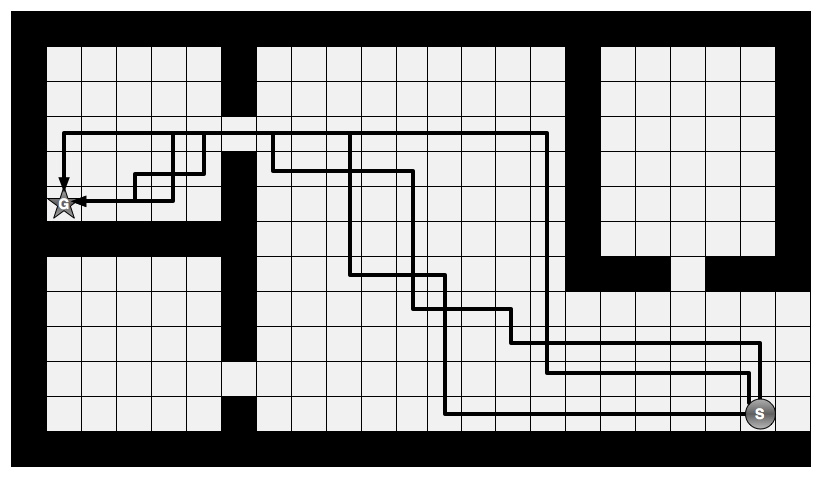
\includegraphics[scale=0.30, trim = 10mm 10mm 10mm 0mm]{chapter_rsr/diagrams/symmetry.png}
\end{center}
\vspace{-3pt}
\caption{A highly symmetric pathfinding instance. Many solutions exist; we highlight three. }
\label{fig::rsr::symmetry}
\end{figure}

As an illustrative example consider Figure~\ref{fig::rsr::symmetry}. Notice that although there 
is only a single optimal length path this path has many symmetric variations. 
Suppose we run an optimal algorithm such as A* to solve this problem. Notice that each time 
we expand a node $n$ we need to expand all nodes on the path to $n$. Moreover, if we assume an 
unfavourable tie-breaking strategy, we will also need to expand every node on symmetric path 
to $n$. In a worst-case we may expand a majority of all nodes from the map.

